\documentclass{beamer}
\usepackage[utf8]{inputenc}
\usepackage[american]{babel}
\usetheme{metropolis}
\usepackage{graphicx}
\usepackage{hyperref}
\usepackage{comment}
\usepackage{diagbox}
\usepackage{multirow}
\usepackage{array}
\usepackage{tikz}
\usetikzlibrary{arrows.meta,positioning}

\usepackage [autostyle, english = american]{csquotes}

\MakeOuterQuote{"}

\setbeamerfont{bibliography item}{size=\tiny}
\setbeamerfont{bibliography entry author}{size=\tiny}
\setbeamerfont{bibliography entry title}{size=\tiny}
\setbeamerfont{bibliography entry location}{size=\tiny}
\setbeamerfont{bibliography entry note}{size=\tiny}

\definecolor{themecolor}{RGB}{0,116,178}
\setbeamercolor{title}{fg=themecolor}
\setbeamercolor{structure}{fg=themecolor}
\setbeamercolor{section}{fg=themecolor}
\setbeamercolor{frametitle}{fg=white, bg=themecolor}
\setbeamercolor{background canvas}{bg=white}

\newcommand{\imp}[1]{\textbf{\color{cyan}#1}}
\newcommand{\de}[1]{\textbf{\color{red}#1}}
\newcommand{\source}[1]{%
	\vfill
	{\tiny\color{gray}#1}
}

\newcommand{\TeaserImage}[1]{\raisebox{%
		.5\dimexpr-\height+\ht\strutbox-\dp\strutbox}{%
		\includegraphics[width=0.15\textwidth]{#1}}}

\hypersetup{
	colorlinks=true,
	linkcolor=themecolor,
	filecolor=magenta,      
	urlcolor=cyan,
}

\metroset{block=fill}

\title{Refining the Computational Analysis of Interactive Fiction: A Hybrid Framework using Bag-of-Paths 
Formalism and LLMs}
\date{}
\author{Guillaume Guex \href{mailto:guillaume.guex@unil.ch}{\texttt{guillaume.guex@unil.ch}}}
\institute{University of Lausanne}

\begin{document}
	
  	\maketitle

	%-------------------------------------------%
  		
  	\section{Introduction}
  	
  	%-------------------------------------------%
  	
	\begin{frame}{Interactive Fictions and Gamebooks}
		\footnotesize
		An \imp{interactive fiction} is a form of narrative in which the reader’s or player’s choices influence the sequence of events, the accessible content, or the story’s outcome. \\
		\vspace{0.1cm}
		A \imp{gamebook} is a book-based form of interactive fiction, usually divided into numbered sections connected by choices, rules, and sometimes game mechanics such as combat, inventory, or chance.
		
		\begin{center}
			\fbox{
			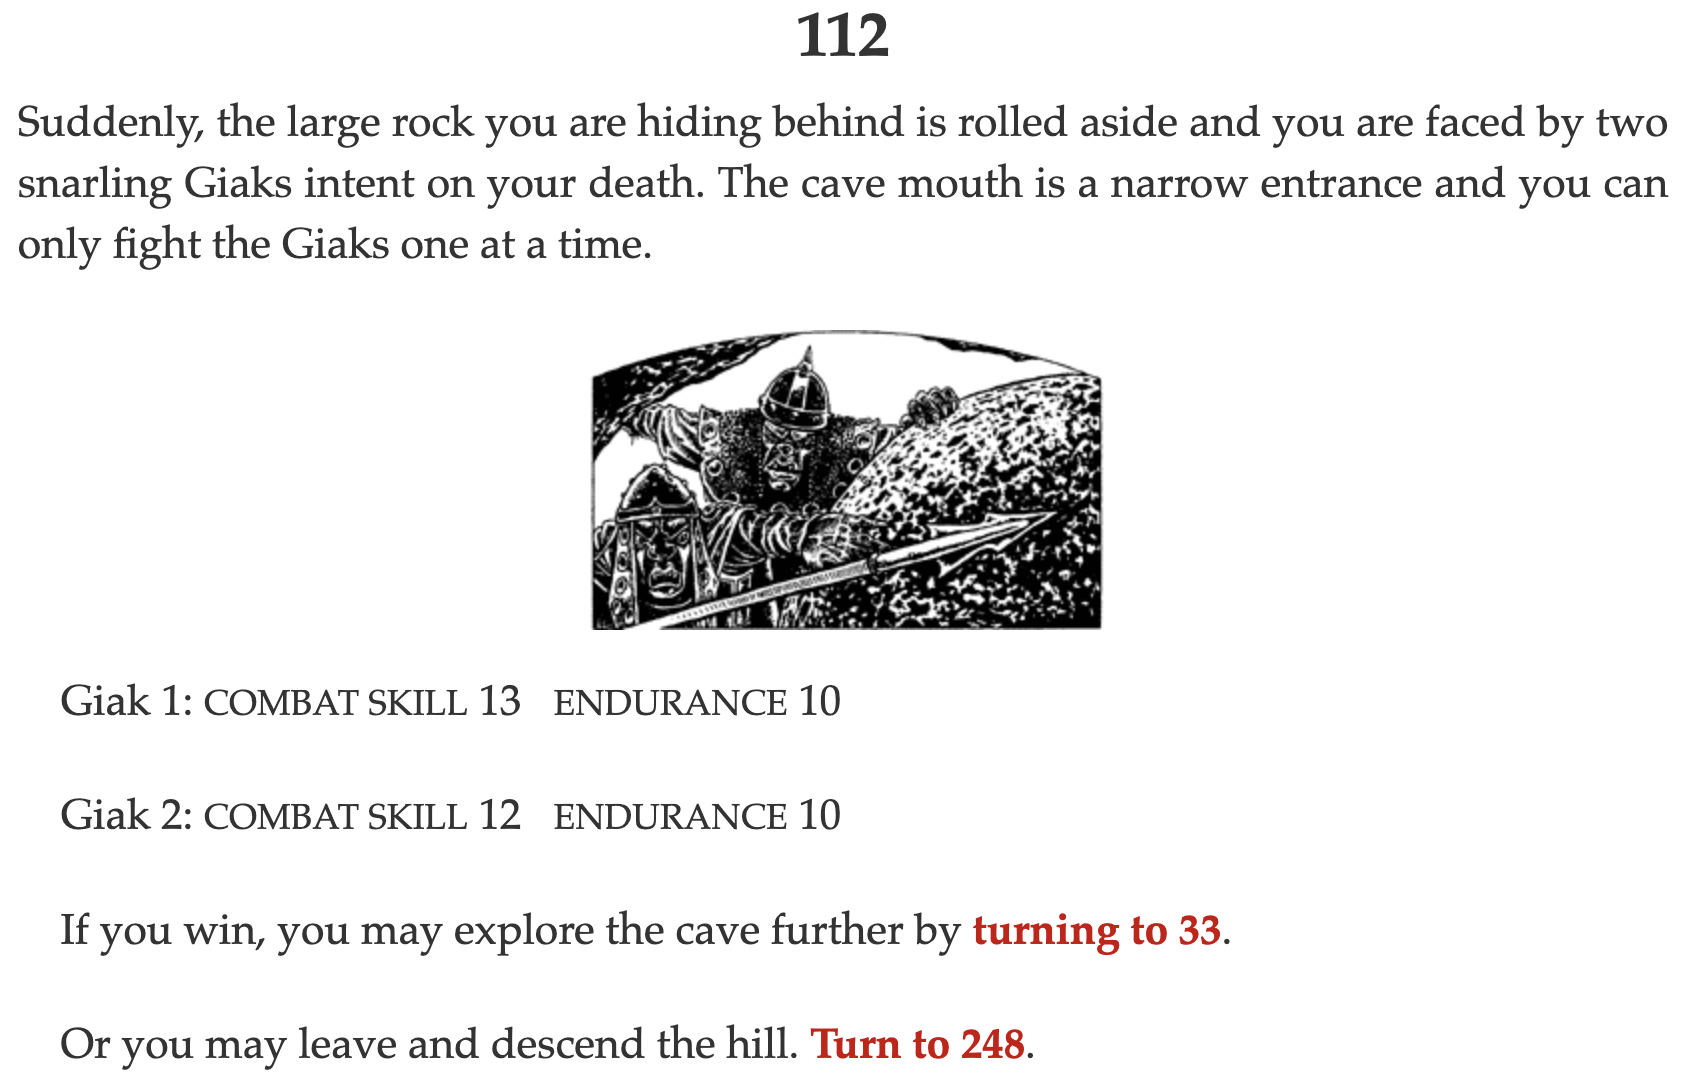
\includegraphics[width=0.8\textheight]{fig/LW01_112.png}
			} \\
			{\tiny \textit{Flight from the Dark} by Joe Dever and Gary Chalk \href{www.projectaon.org}{www.projectaon.org}}
		\end{center}
	\end{frame}
  	
  	%-------------------------------------------%
  	
  	\begin{frame}{The classical representation: a graph}
  		Interactive fiction is traditionally modeled as a
  		\imp{directed graph}.
  	\begin{columns}[T]
  		\begin{column}{0.55\textwidth}			 			
  			\vspace{0.4cm}
  			
  			\begin{itemize}
  				\item \imp{Nodes} represent \emph{paragraphs}, i.e. numbered narrative sections.
  				\item \imp{Edges} represent \emph{transitions}, i.e. the choices available to the player.
  			\end{itemize}
  		\end{column}
  		
  		\begin{column}{0.45\textwidth}
  			\centering
  			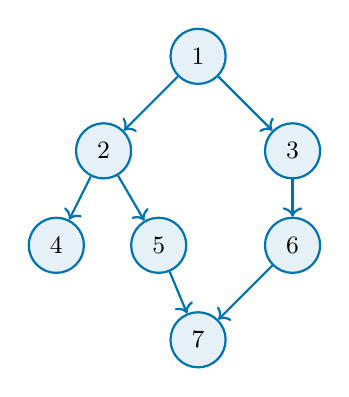
\begin{tikzpicture}[
  				node/.style={
  					circle,
  					draw=themecolor,
  					thick,
  					fill=themecolor!10,
  					minimum size=7mm,
  					font=\small
  				},
  				edge/.style={
  					->,
  					thick,
  					draw=themecolor
  				}
  				]
  				\node[node] (a) at (0,0) {1};
  				\node[node] (b) at (-1.2,-1.2) {2};
  				\node[node] (c) at (1.2,-1.2) {3};
  				\node[node] (d) at (-1.8,-2.4) {4};
  				\node[node] (e) at (-0.5,-2.4) {5};
  				\node[node] (f) at (1.2,-2.4) {6};
  				\node[node] (g) at (0,-3.6) {7};
  				
  				\draw[edge] (a) -- (b);
  				\draw[edge] (a) -- (c);
  				\draw[edge] (b) -- (d);
  				\draw[edge] (b) -- (e);
  				\draw[edge] (c) -- (f);
  				\draw[edge] (e) -- (g);
  				\draw[edge] (f) -- (g);
  			\end{tikzpicture}
  		\end{column}
  		\end{columns}
  		
  		\vfill
  		
  		The \imp{Main limitation} of this representation : 
  		\begin{itemize}
  			\item The \imp{structure} or the \imp{topology} of the work can be studied. 
  			\item The text itself, therefore the \imp{narrative meaning}, is no longer taken into account.
  		\end{itemize}
  		
  	\end{frame}
  	
  	%-------------------------------------------%
  	
  	\begin{frame}{A hybrid solution: graphs and LLMs}
  		\scriptsize
  		\imp{Large Language Models (LLM)} make it possible to reintroduce the semantic content discarded by graph modeling. 
  		\begin{block}{\scriptsize \de{Our approach : both methods}}
  			\begin{itemize}
  				\item The \imp{graph} models the \imp{structure} of the work
  				\item The \imp{LLM} interprets the \imp{narrative content}
  			\end{itemize}
  		\end{block}
  		
  		
  		\begin{center}
  			\scalebox{0.7}{
  			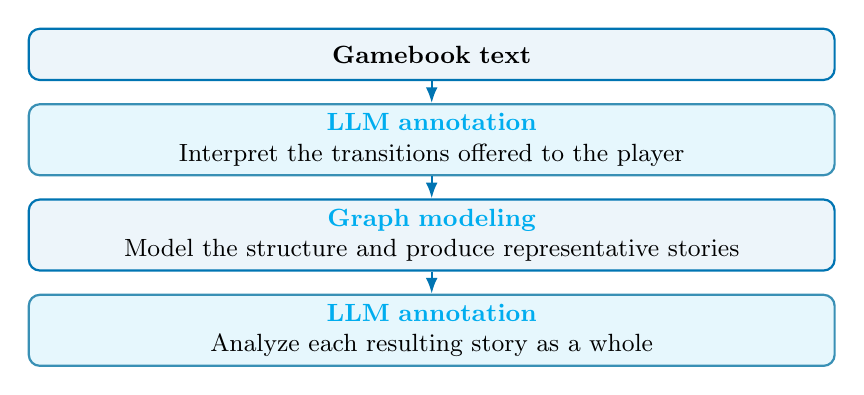
\begin{tikzpicture}[
  				stagebox/.style={
  					rounded corners,
  					draw=themecolor,
  					fill=themecolor!7,
  					thick,
  					minimum height=0.65cm,
  					text width=10cm,
  					align=center,
  					font=\small
  				},
  				llmbox/.style={
  					rounded corners,
  					draw=cyan!70!black,
  					fill=cyan!10,
  					thick,
  					minimum height=0.65cm,
  					text width=10cm,
  					align=center,
  					font=\small
  				},
  				flowarrow/.style={
  					-{Latex[length=2mm]},
  					thick,
  					draw=themecolor
  				},
  				node distance=0.28cm
  				]
  				
  				\node[stagebox] (text) {
  					\textbf{Gamebook text}
  				};
  				
  				\node[llmbox, below=of text] (local) {
  					\textbf{\imp{LLM annotation}}\\
  					Interpret the transitions offered to the player
  				};
  				
  				\node[stagebox, below=of local] (graph) {
  					\textbf{\imp{Graph modeling}}\\
  					Model the structure and produce representative stories
  				};
  				
  				\node[llmbox, below=of graph] (global) {
  					\textbf{\imp{LLM annotation}}\\
  					Analyze each resulting story as a whole
  				};
  				
  				\draw[flowarrow] (text) -- (local);
  				\draw[flowarrow] (local) -- (graph);
  				\draw[flowarrow] (graph) -- (global);
  				
  			\end{tikzpicture}
  			}
  		\end{center}
  		
  		\begin{block}{\de{\scriptsize Research question}}
  			How can graph modeling and local LLM annotation be combined to study
  			both the structural possibilities and the narrative experiences
  			produced by a gamebook?
  		\end{block}
  		
  	\end{frame}
  	
  	%-------------------------------------------%
  	
  	\begin{frame}{Methodogical choice : local LLM}
  		
  		\scriptsize
  		
  		\begin{block}{\de{Methodological choice}}
  			\begin{itemize}
  				\item We are going to use exclusively \imp{Qwen3.6-27B}, executed locally on university infrastructure. 
  				\item The local model is not treated as an autonomous literary critic.
  				It is used as a \imp{controlled annotation instrument} whose
  				decisions remain open to inspection.
  			\end{itemize}
  		\end{block}
  		
  		\begin{columns}[T,onlytextwidth]
  			\scriptsize
  			\begin{column}[T]{0.48\textwidth}
  				\vspace{0pt}
  				\textbf{Methodological reasons}
  				
  				\begin{itemize}
  					\item No dependency on a proprietary API
  					\item Prompts and inference settings are documented
  					\item Outputs can be stored, inspected and reproduced
  					\item Source texts remain on local infrastructure
  					\item Lower and predictable financial cost
  				\end{itemize}
  			\end{column}
  			
  			\begin{column}[T]{0.48\textwidth}
  				\vspace{0pt}
  				\textbf{Why is it sufficient?}
  				
  				\begin{itemize}
  					\item The task is a constrained annotation task
  					\item Categories are defined by an explicit codebook
  					\item Outputs follow a restricted JSON schema
  					\item Results are checked against human annotations
  					\item Frontier-level generative capabilities are overkill
  				\end{itemize}
  			\end{column}
  			
  		\end{columns}
  		
  		\vfill
  		
  	\end{frame}
  	
  	%-------------------------------------------%
  	
  	\begin{frame}{Corpus: \emph{Lone Wolf} and Project Aon}
  		\footnotesize
  		The studied corpus is the \imp{Lone Wolf series} created by Joe Dever. 
  		
  		The \imp{project Aon} (\href{www.projectaon.org}{www.projectaon.org}) provides authorized digital editions of the books. It is already structured with html. 
  		
  		There are \imp{several mechanics} in these gamebooks : 
  		\begin{columns}
  			\begin{column}[T]{0.48\textwidth}
  				\begin{itemize}
	  				\item Branching choices and forced transitions
	  				\item Random events
	  				\item Player profile with stats and special powers
	  				\item Combat with possible evasion
	  			\end{itemize}
  			\end{column}
  			\begin{column}[T]{0.48\textwidth}
  				\begin{itemize}
	  				\item Endurance (HP) management
	  				\item Items and inventory management
	  				\item Puzzles and hidden links
	  			\end{itemize}
  			\end{column}
  		\end{columns}
  		
  		\begin{block}{ \footnotesize \de{Scope of this presentation}}
  			A complete representation of every mechanic would make the model
  			intractable.  We use \imp{explicit simplifications} and focus
  			exclusively on \imp{Book 1: \emph{Flight from the Dark}}.
  		\end{block}
  		
  	\end{frame}
  	
  	%-------------------------------------------%
  	
  	\begin{frame}{Modeling scope: from L0 to L3}
  		\footnotesize
  		The goal is to build a tractable \imp{Markovian model}: for a fixed player profile, the next transition depends only on the current node, not on the complete play history.
  		
  		\vspace{0.15cm}
  		
  		\begin{center}
  			\tiny
	  		\begin{tabular}{|c|c|p{0.43\textwidth}|c|}
	  			
	  			\hline
	  			
	  			\textbf{Level} &
	  			\textbf{Information} &
	  			\textbf{Mechanics} &
	  			\textbf{Decision} \\
	  			
	  			\hline
	  			
	  			\textbf{L0} &
	  			Topology &
	  			Paragraphs, links, forced transitions, Death and Win outcomes &
	  			\textcolor{green!50!black}{\textbf{Included}} \\
	  			
	  			\hline
	  			
	  			\textbf{L1} &
	  			Player agency &
	  			Choices annotated along the risk, morality and action axes &
	  			\textcolor{green!50!black}{\textbf{Included}} \\
	  			
	  			\hline
	  			
	  			\textbf{L2} &
	  			Uncertainty &
	  			Random events, combat, evasion, Kai Disciplines (special powers) and conditions &
	  			\textcolor{orange!80!black}{\textbf{Simplified}} \\
	  			
	  			\hline
	  			
	  			\textbf{L3} &
	  			Persistent state &
	  			Endurance, healing, inventory, gold, equipment and meals &
	  			\textcolor{red!75!black}{\textbf{Not simulated}} \\
	  			
	  			\hline
	  		\end{tabular}
  		\end{center}
  		
  		\imp{L2 simplifications} :
  		\begin{itemize}
  			\item One global combat-win probability
  			\item One global escape probability
  			\item Kai Disciplines availability fixed at $0.5$
  			\item One generic \texttt{has\_condition} probability
  		\end{itemize}
  	\end{frame}
  	
  	%-------------------------------------------%
  	
  	\begin{frame}{Outline of the presentation}
  		\scriptsize
  		\imp{1. Paragraph parsing and transition annotation}
  		
  		A local LLM reads the choices offered at each paragraph and outputs :
  		\begin{itemize}
  			\item Transition types
  			\item Game mechanics
  			\item Risk, morality and action labels
  		\end{itemize}
  		
  		\imp{2. Graph modeling and Bag-of-Path formalism}
  		
  		The annotations are compiled into weighted graphs for different player profiles, and various objects are computed : 
  		\begin{itemize}
  			\item Bag-of-Paths indices
  			\item Local and global measures
  			\item Representative trajectories
  		\end{itemize}
  		
  		\imp{3. Trajectory annotation}
  		
  		A local LLM reads the stories associated with selected
  		trajectories and produce : 
  		\begin{itemize}
  			\item Whole-story annotations
  			\item Profile manifestation
  			\item Pairwise comparisons
  		\end{itemize}
  		
  	\end{frame}
  	
  	%-------------------------------------------%
  	
  	\section{Paragraph parsing and transition annotation}
  	
  	%-------------------------------------------%
  	
  	\begin{frame}{Objective: from paragraphs to structured data}
  		
  		\begin{block}{\de{Objective}}
  			\small
  			Transform each gamebook paragraph into an
  			\imp{structured representation}, separating
  			\imp{narrative units} from the \imp{transitions} offered to the player.
  		\end{block}
  		
  		\vspace{0.1cm}
  		
  		\begin{columns}[T,onlytextwidth]
  			
  			\begin{column}[T]{0.29\textwidth}
  				\vspace{0pt}
  				\centering
  				\textbf{Project Aon page}
  				
  				\vspace{0.1cm}
  				
  				\fbox{%
  					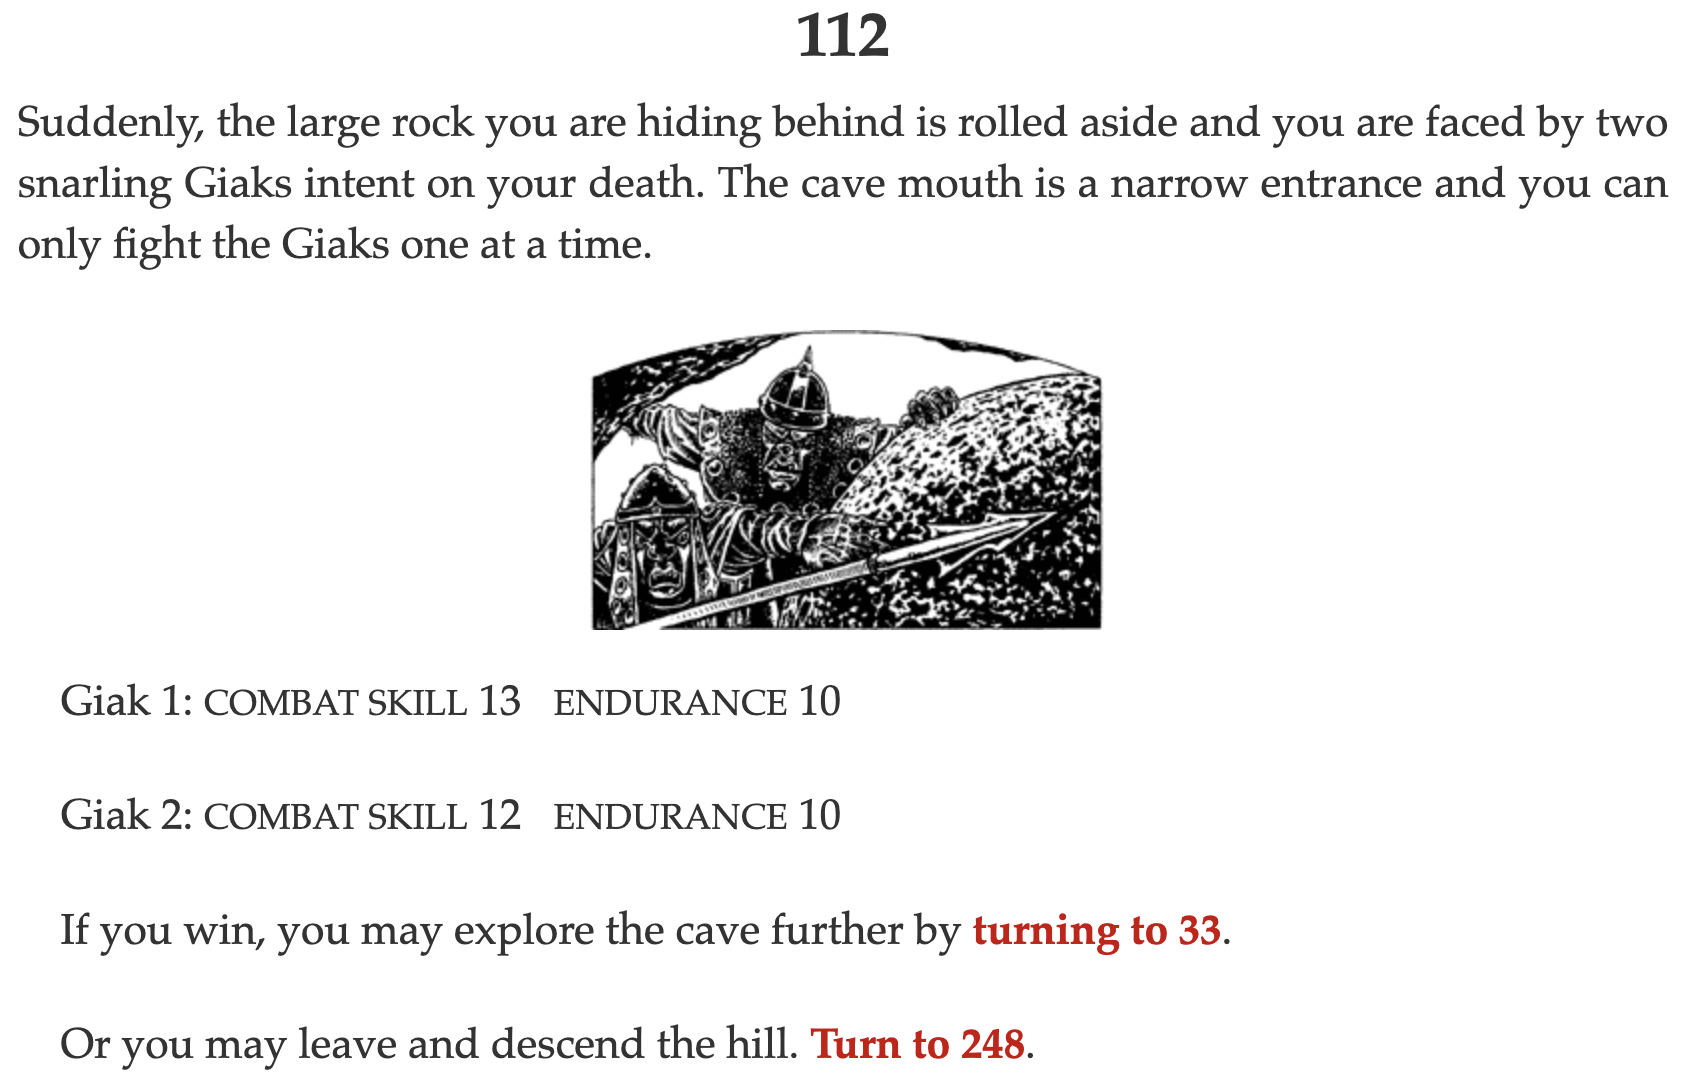
\includegraphics[
  					width=0.92\linewidth,
  					height=0.49\textheight,
  					keepaspectratio
  					]{fig/LW01_112.png}%
  				}
  				
  				\vspace{0.1cm}
  				
  				{\tiny Paragraph 112}
  			\end{column}
  			
  			\begin{column}[T]{0.11\textwidth}
  				\vspace{1.5cm}
  				\centering
  				
  				{\Large $\Longrightarrow$}
  				
  				\vspace{0.1cm}
  				
  				{\tiny Parsing\\+\\ \vspace{-0.2cm}LLM}
  			\end{column}
  			
  			\begin{column}[T]{0.56\textwidth}
  				\vspace{0pt}
  				\centering
  				
  				\textbf{\texttt{LW01\_nodes.csv}}
  				
  				\vspace{0.1cm}
  				
  				{\tiny
  					\resizebox{\linewidth}{!}{%
  						\begin{tabular}{|c|c|c|c|}
  							\hline
  							\texttt{node\_id} &
  							\texttt{text\_content} &
  							\texttt{absorbing\_status} &
  							\texttt{enemies} \\
  							\hline
  							112 &
  							Suddenly, the large rock\ldots &
  							\texttt{potential\_death} &
  							Giak 1; Giak 2 \\
  							\hline
  						\end{tabular}
  				}}
  				
  				\vspace{0.5cm}
  				
  				\centering
  				\textbf{\texttt{LW01\_edges.csv}}
  				
  				\vspace{0.1cm}
  				
  				% First half of the columns
  				{\tiny
  					\resizebox{\linewidth}{!}{%
  						\begin{tabular}{|c|c|c|c|c|}
  							\hline
  							\texttt{source\_id} &
  							\texttt{target\_id} &
  							\texttt{edge\_text} &
  							\texttt{transition\_type} &
  							\texttt{realisation\_value} \\
  							\hline
  							
  							112 &
  							33 &
  							If you win, explore the cave\ldots &
  							\texttt{explicit\_choice} &
  							\texttt{If you win} \\
  							
  							\hline
  							
  							112 &
  							248 &
  							Leave and descend the hill\ldots &
  							\texttt{explicit\_choice} &
  							\texttt{If you win} \\
  							
  							\hline
  						\end{tabular}%
  				}}
  				
  				\vspace{0.15cm}
  				
  				% Second half of the columns
  				{\tiny
  					\resizebox{\linewidth}{!}{%
  						\begin{tabular}{|c|c|c|c|c|c|}
  							\hline
  							\texttt{source\_id} &
  							\texttt{target\_id} &
  							\texttt{semantic\_risk} &
  							\texttt{semantic\_morality} &
  							\texttt{semantic\_action} &
  							\texttt{warnings} \\
  							\hline
  							
  							112 &
  							33 &
  							\texttt{reckless} &
  							\texttt{neutral} &
  							\texttt{tactical} &
  							-- \\
  							
  							\hline
  							
  							112 &
  							248 &
  							\texttt{cautious} &
  							\texttt{selfish} &
  							\texttt{physical} &
  							-- \\
  							
  							\hline
  						\end{tabular}%
  				}}
  				
  				\vspace{0.1cm}
  				
  			\end{column}
  			
  		\end{columns}
  		
  		
  		
  	\end{frame}
  	
  	%-------------------------------------------%
  	
	\begin{frame}{Rule-based parsing versus LLM-based annotations}
		\scriptsize
		\imp{Rule-based parsing (on html)}
		
		Can process all fields in the \imp{node table}, and \imp{some fields in the edges tables} (\texttt{source\_id}, \texttt{target\_id}, and
		\texttt{edge\_text}, used for validation).
		
		\vspace{0.1cm}
		
		\imp{LLM-based annotations}
		
		All fields in the \imp{edge table}, in particular :
		
		\begin{itemize}
			\item Transition mechanism:
			\texttt{transition\_type}, \texttt{realisation\_value};
			\item Meaning of player choices:
			\texttt{semantic\_risk}, \texttt{semantic\_morality},
			\texttt{semantic\_action};
			\item Ambiguities requiring attention:
			\texttt{warnings}.
		\end{itemize}
		
		\begin{block}{\scriptsize \de{Methodological choice}}
			Each explicit player choice is annotated according to \imp{3 independent semantic axes} : 
			
			\begin{itemize}
				\item \imp{Risk}: exposure to danger (cautious, neutral, reckless)
				\item \imp{Morality} : treatment of others (selfish, neutral, noble)
				\item \imp{Action} : mode of intervention (physical, neutral, tactical)
			\end{itemize}
		\end{block}
	\end{frame}
	
	%-------------------------------------------%
	
	\begin{frame}{From prompt to structured annotation}
		
		\centering
		
		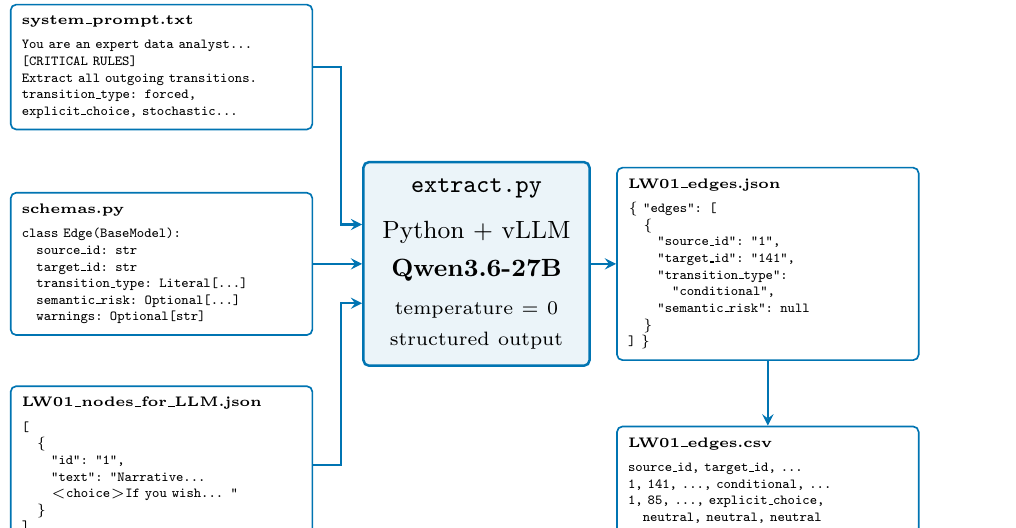
\begin{tikzpicture}[
			file/.style={
				draw=themecolor,
				line width=0.6pt,
				rounded corners=2pt,
				fill=white,
				align=left,
				inner sep=4pt,
				font=\ttfamily\tiny
			},
			engine/.style={
				draw=themecolor,
				line width=0.9pt,
				rounded corners=2pt,
				fill=themecolor!8,
				align=center,
				inner sep=6pt,
				font=\small
			},
			flow/.style={
				->,
				>=stealth,
				line width=0.8pt,
				draw=themecolor
			}
			]
			
			\useasboundingbox (-6.1,-3.0) rectangle (6.1,3.0);
			
			% Prompt
			\node[file,text width=3.55cm] (prompt) at (-4.4,2.5) {%
				{\bfseries\rmfamily system\_prompt.txt}\\[1mm]
				You are an expert data analyst...\\
				\textbf{[CRITICAL RULES]}\\
				Extract all outgoing transitions.\\
				\texttt{transition\_type}: forced,\\
				explicit\_choice, stochastic...
			};
			
			% Schema
			\node[file,text width=3.55cm] (schema) at (-4.4,0) {%
				{\bfseries\rmfamily schemas.py}\\[1mm]
				class Edge(BaseModel):\\
				\quad source\_id: str\\
				\quad target\_id: str\\
				\quad transition\_type: Literal[...]\\
				\quad semantic\_risk: Optional[...]\\
				\quad warnings: Optional[str]
			};
			
			% Input corpus
			\node[file,text width=3.55cm] (corpus) at (-4.4,-2.55) {%
				{\bfseries\rmfamily LW01\_nodes\_for\_LLM.json}\\[1mm]
				[\\
				\quad \{\\
				\qquad \char34 id\char34: \char34 1\char34,\\
				\qquad \char34 text\char34: \char34 Narrative...\\
				\qquad \textless choice\textgreater If you wish... \char34\\
				\quad \}\\
				]
			};
			
			
			% Python + LLM
			\node[engine,text width=2.45cm] (engine) at (-0.4,0) {%
				\textbf{\texttt{extract.py}}\\[2mm]
				Python + vLLM\\[1mm]
				\textbf{Qwen3.6-27B}\\[2mm]
				\scriptsize
				temperature = 0\\
				structured output
			};
			
			% JSON response
			\node[file,text width=3.55cm] (json) at (3.3,0) {%
				{\bfseries\rmfamily LW01\_edges.json}\\[1mm]
				\{ \char34 edges\char34: [\\
				\quad \{\\
				\qquad \char34 source\_id\char34: \char34 1\char34,\\
				\qquad \char34 target\_id\char34: \char34 141\char34,\\
				\qquad \char34 transition\_type\char34:\\
				\qquad \quad \char34 conditional\char34,\\
				\qquad \char34 semantic\_risk\char34: null\\
				\quad \}\\
				] \}
			};
			
			% Final CSV
			\node[file,text width=3.55cm] (csv) at (3.3,-2.75) {%
				{\bfseries\rmfamily LW01\_edges.csv}\\[1mm]
				source\_id, target\_id, ...\\
				1, 141, ..., conditional, ...\\
				1, 85, ..., explicit\_choice,\\
				\quad neutral, neutral, neutral
			};
			
			% Input arrows
			\draw[flow]
			(prompt.east) -- ++(0.35,0)
			|- ([yshift=5mm]engine.west);
			
			\draw[flow]
			(schema.east) -- (engine.west);
			
			\draw[flow]
			(corpus.east) -- ++(0.35,0)
			|- ([yshift=-5mm]engine.west);
			
			% Output arrows
			\draw[flow]
			(engine.east) -- (json.west);
			
			\draw[flow]
			(json.south) -- (csv.north);
			
		\end{tikzpicture}
		
	\end{frame}
	
	%-------------------------------------------%
	
	\begin{frame}{Iterative prompt refinement}
		\footnotesize
		\centering
		
		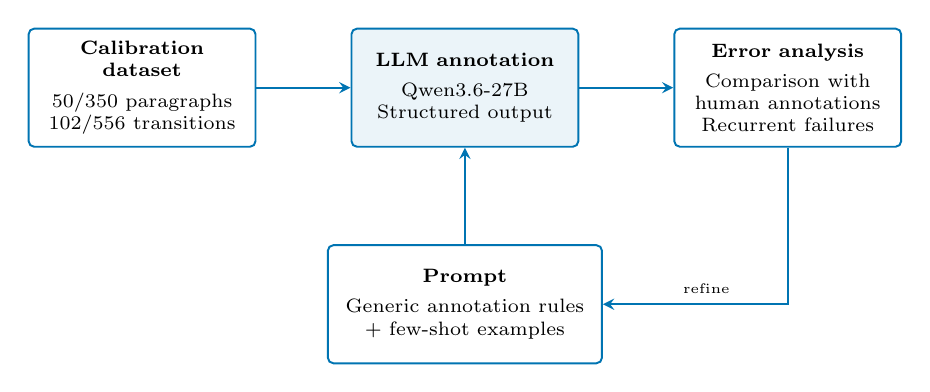
\begin{tikzpicture}[
			calbox/.style={
				draw=themecolor,
				rounded corners=2pt,
				line width=0.7pt,
				fill=white,
				align=center,
				text width=2.6cm,
				minimum height=1.5cm,
				inner sep=4pt,
				font=\scriptsize
			},
			calarrow/.style={
				->,
				>=stealth,
				draw=themecolor,
				line width=0.8pt
			}
			]
			
			% First line
			\node[calbox] (human) at (-4.1,1.5) {
				\textbf{Calibration dataset}\\[1mm]
				50/350 paragraphs\\
				102/556 transitions
			};
			
			\node[calbox,fill=themecolor!8] (llm) at (0,1.5) {
				\textbf{LLM annotation}\\[1mm]
				Qwen3.6-27B\\
				Structured output
			};
			
			\node[calbox] (errors) at (4.1,1.5) {
				\textbf{Error analysis}\\[1mm]
				Comparison with human annotations\\
				Recurrent failures
			};
			
			% Second line
			\node[calbox,text width=3.2cm] (prompt) at (0,-1.25) {
				\textbf{Prompt}\\[1mm]
				Generic annotation rules\\
				+ few-shot examples
			};
			
			% Main sequence
			\draw[calarrow]
			(human.east) --
			(llm.west);
			
			\draw[calarrow]
			(llm.east) --
			(errors.west);
			
			% Prompt injection
			\draw[calarrow]
			(prompt.north) --
			(llm.south);
			
			% Refinement loop
			\draw[calarrow]
			(errors.south) |-
			node[pos=0.72,above,font=\tiny]{refine}
			(prompt.east);
			
		\end{tikzpicture}
		
		\vspace{0.4cm}
		
		\begin{itemize}
			\item Errors lead to revisions of \imp{general annotation rules},
			not paragraph-specific corrections.
			\item This iterative process is a \imp{calibration}, not an
			independent evaluation.
			\item No held-out validation set was used because of limited time;
			generalization to another book is therefore not measured.
		\end{itemize}
		
	\end{frame}
	
	%-------------------------------------------%
	
	\begin{frame}{Annotation results}
		\footnotesize
		
		\imp{Calibration} : On 50 paragraphs and 102 transitions, the final prompt produced no
		missing or invented transition and no transition-type disagreement. Only 3 (on 177 annotations) semantic disagreements : two for risk and one for action.
		
		\begin{center}
			\imp{Paragraph statistics}
			
			
			\scalebox{0.7}{
				\begin{tabular}{|l|c|}
					
					\hline
					Total & 350 \\
					Terminal & 16 deaths / 1 victory \\
					One outgoing transitions & 157 \\
					Two outgoing transitions & 134 \\
					Three or more outgoing transitions & 42 \\
					Paragraphs with enemies & 29 \\
					\hline
				\end{tabular}
			}
			
			\vspace{0.3cm}
			\imp{Transition statistics}
			\vspace{-0.3cm}
		\end{center}
		
		\begin{columns}[T,onlytextwidth]
			
			\begin{column}{0.32\textwidth}
				\centering
				\scalebox{0.7}{
				\begin{tabular}{|l|r|r|}
					\hline
					\textbf{Transition type} & \textbf{N} & \textbf{\%} \\
					\hline
					Explicit choice & 291 & 52.3 \\
					Forced          & 157 & 28.2 \\
					Conditional     & 66  & 11.9 \\
					Stochastic      & 42  & 7.6 \\
					\hline
					\textbf{Total}  & \textbf{556} & \textbf{100.0} \\
					\hline
				\end{tabular}
				}
			\end{column}
			
			\begin{column}{0.64\textwidth}
				\centering
				\scalebox{0.7}{
				\begin{tabular}{|l|l|l|l|}
					\hline
					\textbf{Axis} & \textbf{First pole}
					& \textbf{Neutral} & \textbf{Opposite pole} \\
					\hline
					Risk
					& cautious: 95 (32.6\%)
					& 84 (28.9\%)
					& reckless: 112 (38.5\%) \\
					Morality
					& selfish: 18 (6.2\%)
					& 262 (90.0\%)
					& noble: 11 (3.8\%) \\
					Action
					& physical: 101 (34.7\%)
					& 126 (43.3\%)
					& tactical: 64 (22.0\%) \\
					\hline
				\end{tabular} 
				}
				
				\vspace{0.2cm}
				
				\scalebox{0.7}{
				\begin{tabular}{|l|l|}
					\hline
					Warnings & 53 (9.5\%)  \\
					\hline
				\end{tabular}
				}
			\end{column}
				
		\end{columns}
		
	\end{frame}
	
	%-------------------------------------------%
	
	\begin{frame}{Result of paragraph annotation}
		
		\centering
		
		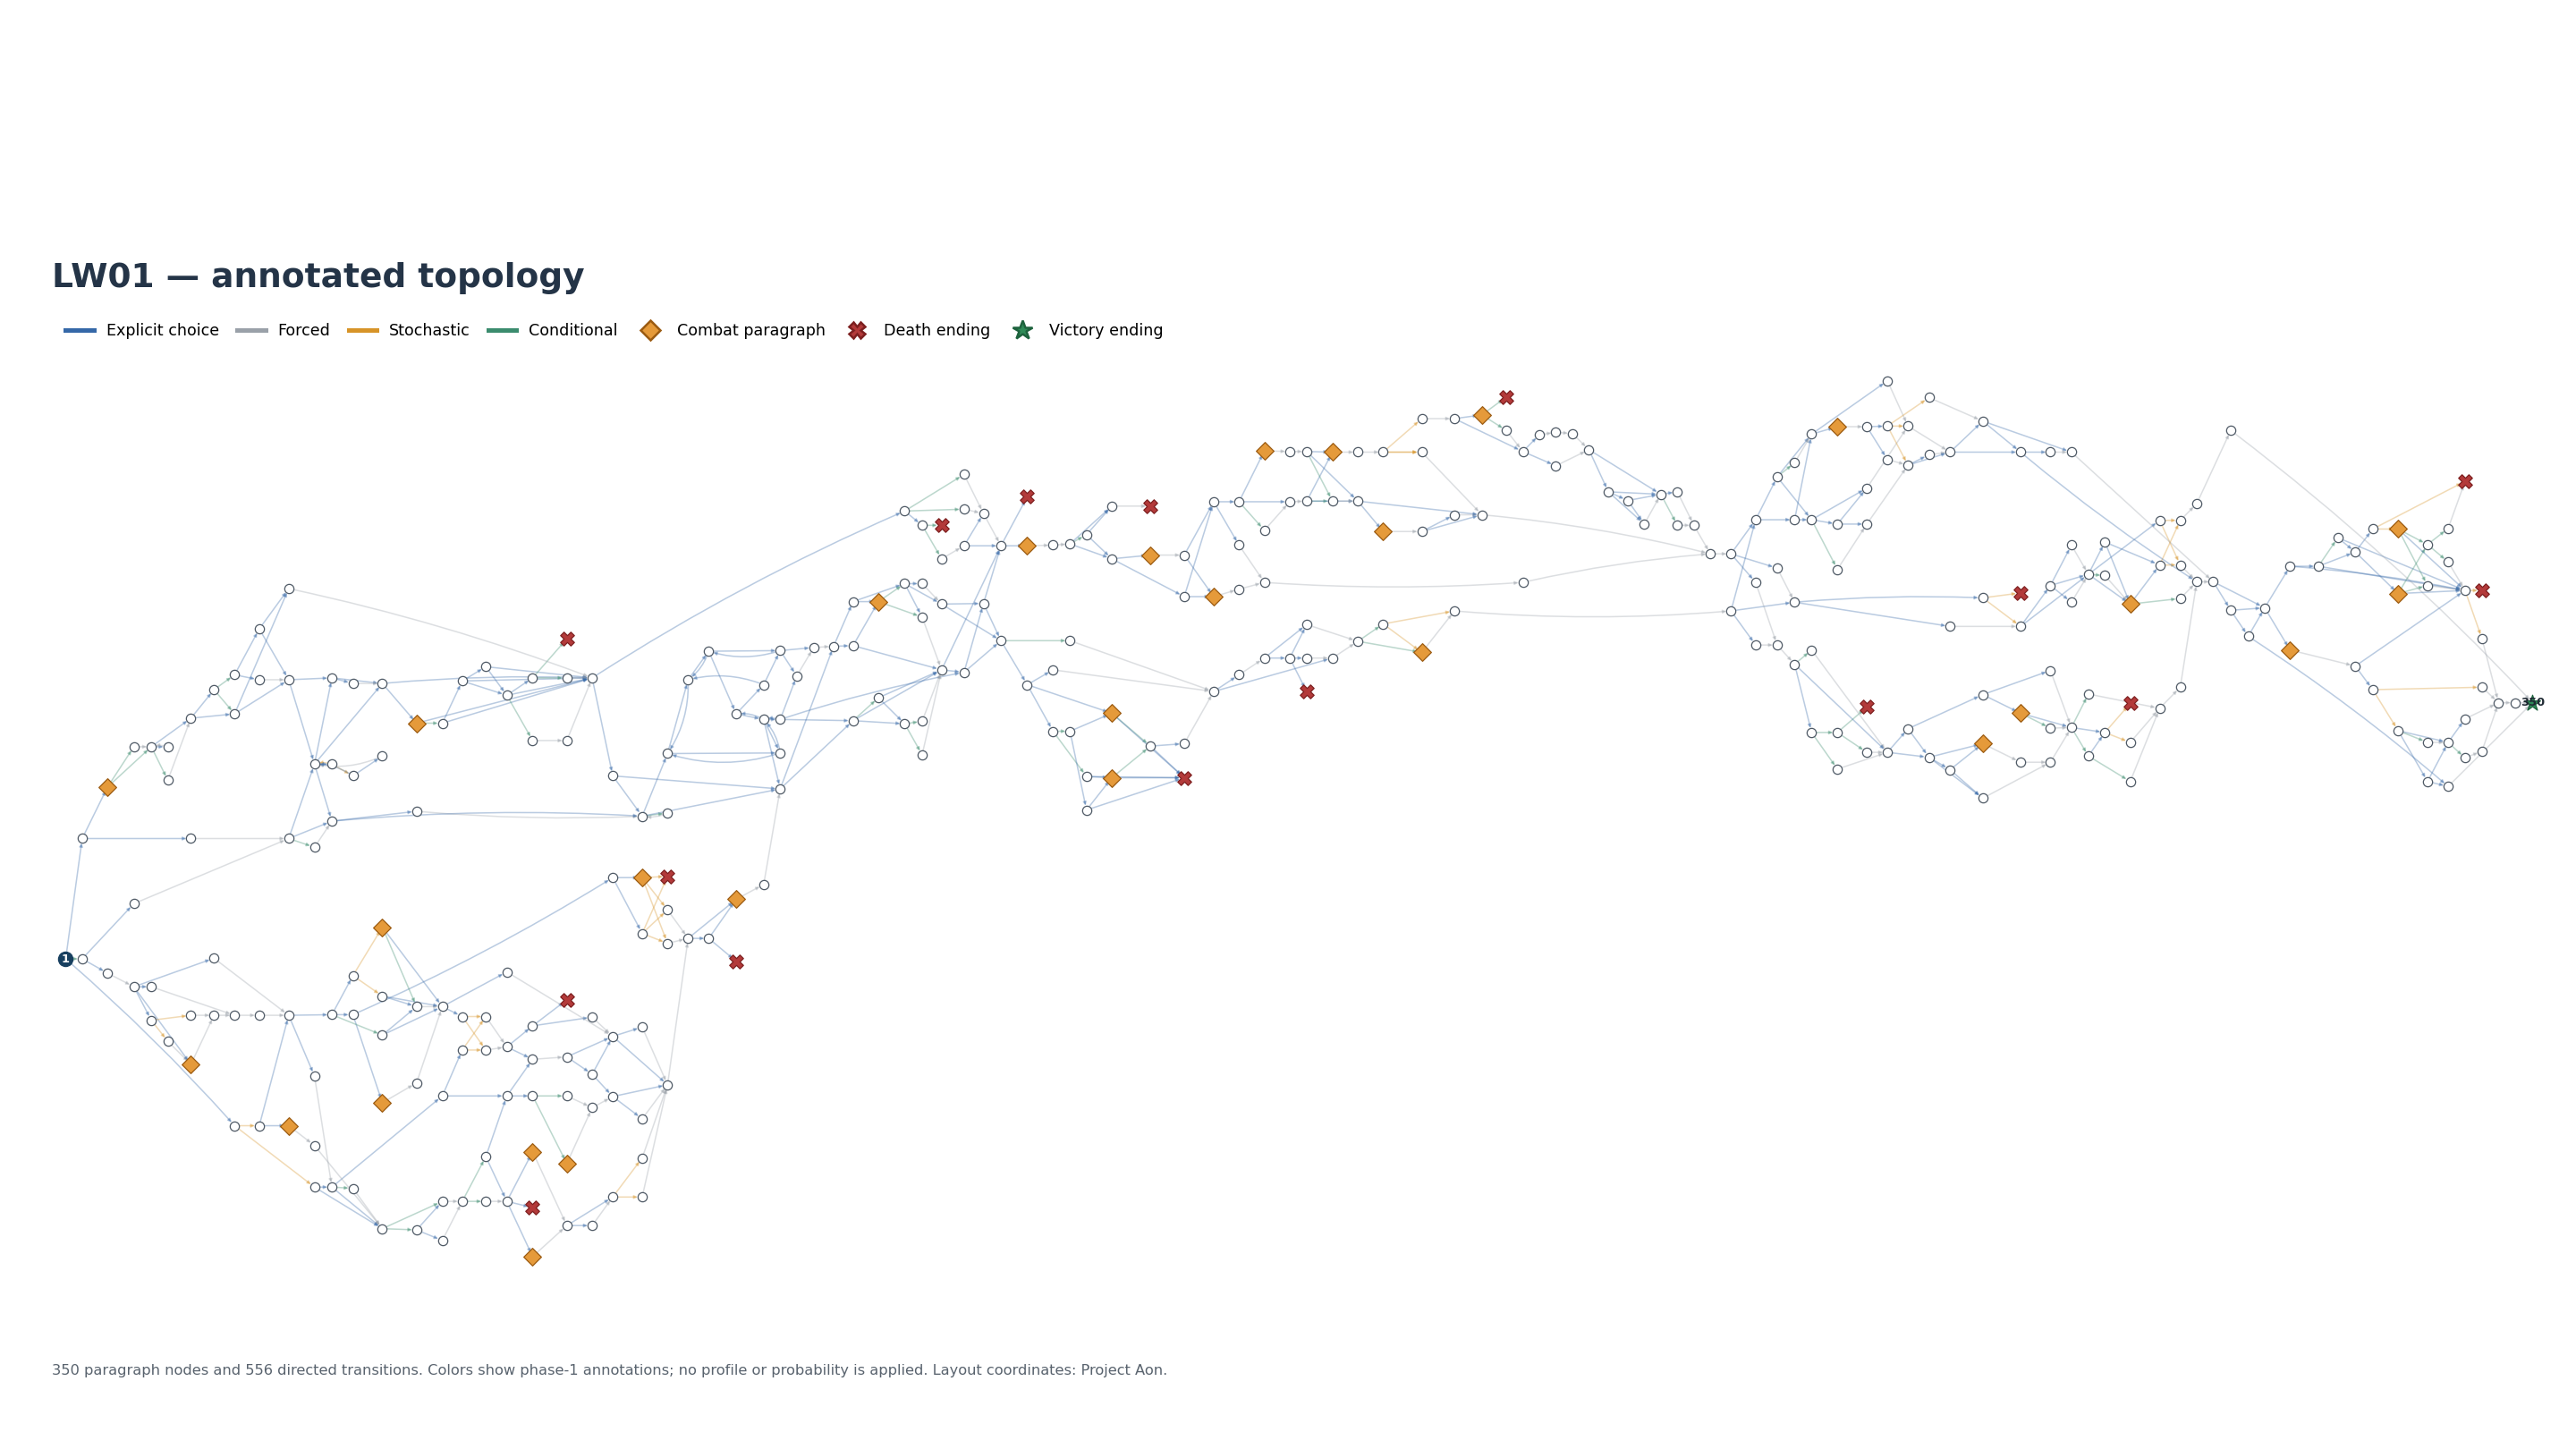
\includegraphics[
		width=\textwidth,
		height=0.78\textheight,
		keepaspectratio
		]{fig/LW01_phase1_unweighted_graph.png}
		
		\vspace{-0.15cm}
		
		{\small
			The topology and transition types are now available, but \imp{transition probabilities depends on player profiles} (next section).
		}
		
	\end{frame}
	
	%-------------------------------------------%
	
	\section{Graph construction and Bag-of-Paths analysis}
	
	%-------------------------------------------%
	
	\begin{frame}{Objective: from annotations to structural measures}
		
		\scriptsize
		
		The objectives here are to : 
		\begin{itemize}
			\item Transform annotations into
			\imp{weighted directed graphs (i.e. a Markov chain matrix)} which depend on \imp{player profiles}.
			\item Compute \imp{various indices with the Bag-of-Path formalism}.
		\end{itemize}
		
		
		\vspace{0.35cm}
		
		\centering
		
		\scalebox{0.7}{
		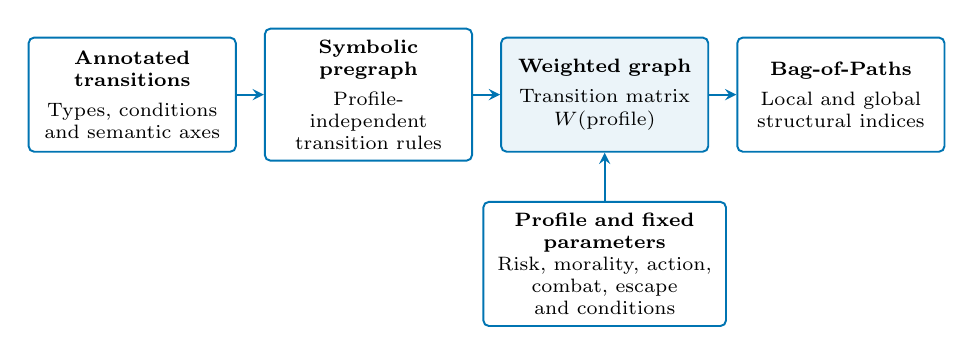
\begin{tikzpicture}[
			graphbox/.style={
				draw=themecolor,
				rounded corners=2pt,
				line width=0.7pt,
				fill=white,
				align=center,
				text width=2.35cm,
				minimum height=1.45cm,
				inner sep=4pt,
				font=\scriptsize
			},
			grapharrow/.style={
				->,
				>=stealth,
				draw=themecolor,
				line width=0.8pt
			}
			]
			
			\node[graphbox] (annotations) at (-4.5,1) {
				\textbf{Annotated transitions}\\[1mm]
				Types, conditions and semantic axes
			};
			
			\node[graphbox] (pregraph) at (-1.5,1) {
				\textbf{Symbolic pregraph}\\[1mm]
				Profile-independent transition rules
			};
			
			\node[graphbox,fill=themecolor!8] (matrix) at (1.5,1) {
				\textbf{Weighted graph}\\[1mm]
				Transition matrix\\
				$W(\mathrm{profile})$
			};
			
			\node[graphbox] (bop) at (4.5,1) {
				\textbf{Bag-of-Paths}\\[1mm]
				Local and global structural indices
			};
			
			\node[graphbox,text width=2.8cm,minimum height=1.1cm]
			(parameters) at (1.5,-1.15) {
				\textbf{Profile and fixed parameters}\\
				Risk, morality, action,\\
				combat, escape and conditions
			};
			
			\draw[grapharrow] (annotations.east) -- (pregraph.west);
			\draw[grapharrow] (pregraph.east) -- (matrix.west);
			\draw[grapharrow] (matrix.east) -- (bop.west);
			\draw[grapharrow] (parameters.north) -- (matrix.south);
			
		\end{tikzpicture}
		}
		
		\vspace{0.1cm}
		
		\raggedright
		
		This section addresses three questions:
		
		\begin{itemize}
			\item How can heterogeneous game mechanics be converted into transition probabilities?
			\item How does the resulting graph vary across player profiles?
			\item Which paragraphs and structural properties are most important across all possible trajectories?
		\end{itemize}
		
	\end{frame}
	
	%-------------------------------------------%
	
	\begin{frame}{One Markov chain per player profile}
		
		\footnotesize
		
		The matrix \imp{$\mathbf{W}^{(p)}$ describes the behavior of one fixed player profile}.
		Once the profile and the experimental parameters are fixed, the next
		transition depends only on the current paragraph.
		
		\vspace{0.2cm}
		
		\begin{columns}[T,onlytextwidth]
			
			\begin{column}{0.47\textwidth}
				\textbf{Player profile}
				
				\vspace{-0.3cm}
				$$
				p=(\text{risk},\text{morality},\text{action})
				$$
				
				{\scriptsize
					\begin{itemize}
						\item Risk: cautious, neutral, reckless
						\item Morality: selfish, neutral, noble
						\item Action: physical, neutral, tactical
					\end{itemize}
				}
				
				\centering
				\imp{$3^3=27$ player profiles}
				
				\vspace{0.25cm}
				
				\raggedright
				\textbf{Fixed parameters (all profiles)}
				
				\vspace{0.05cm}
				
				{\tiny
					\begin{itemize}
						\item Combat victory: $P(\mathrm{win})=0.833$
						\item Combat evasion: $P(\mathrm{escape})=0.5$
						\item Required Kai Discipline available: $P(\mathrm{Kai})=0.5$
						\item Item, gold, or Endurance condition satisfied:
						$P(\mathrm{has\_condition})=0.5$
					\end{itemize}
				}
			\end{column}
			
			\begin{column}{0.49\textwidth}
				\textbf{From profile to probability}
				
				{\scriptsize
					Each choice annotation is compared with the profile:
					\vspace{-0.3cm}
					\begin{center}
						\begin{tabular}{lc}
							\hline
							\textbf{Relation} & \textbf{Affinity} \\
							\hline
							Matching non-neutral values & $2$ \\
							Neutral profile or annotation & $1$ \\
							Opposed non-neutral values & $0.5$ \\
							\hline
						\end{tabular}
					\end{center}
					
					Affinities are multiplied and normalized among the
					available outgoing choices. \\
					\vspace*{0.1cm}
					For a reckless profile facing one reckless and one cautious choice:
					\begin{align*}
						P(\mathrm{reckless})&=\tfrac{2}{2+0.5}=0.8 \\
						P(\mathrm{cautious})&=0.2.
					\end{align*}
				}
			\end{column}
			
		\end{columns}
		
	\end{frame}
	
	%-------------------------------------------%
	
	\begin{frame}{Bag-of-Paths at the Random-Walk limit}
		
		\footnotesize
		
		For each player profile, $\mathbf{W}^{(p)}$ represents the corresponding Markov
		chain. For the BoP calculation, absorbing states have no outgoing
		transitions: $W^{(p)}$ is therefore \imp{substochastic}, and we can compute: 
		$$
		\boxed{
			\mathbf{Z}^{(p)}
			=
			\left(I-\mathbf{W}^{(p)}\right)^{-1}
			=
			I+\mathbf{W}^{(p)}+\left(\mathbf{W}^{(p)}\right)^2+\cdots
		}
		$$
		$z^{(p)}_{si}$ is the \imp{expected number of visits to paragraph $i$
		when starting from paragraph $s$}. Many indices can be derived from the same fundamental matrix : 
		
		\vspace{0.2cm}
		
		\begin{columns}[T,onlytextwidth]
			
			\begin{column}{0.48\textwidth}
				\textbf{Local indices}
				
				{\scriptsize
					Computed for individual paragraphs or transitions:
					
					\begin{itemize}
						\item Probability of visiting a paragraph
						\item Expected visits and edge flows
						\item Contribution to mortality
						\item Impact of a choice on the final outcome
						\item Sensitivity to the player profile
					\end{itemize}
				}
			\end{column}
			
			\begin{column}{0.48\textwidth}
				\textbf{Global indices}
				
				{\scriptsize
					Computed for the complete book and one profile:
					
					\begin{itemize}
						\item Probabilities of victory and death
						\item Expected trajectory length
						\item Total trajectory entropy
						\item Expected coverage and replayability
						\item Divergence between player profiles
					\end{itemize}
				}
			\end{column}
			
		\end{columns}
	\end{frame}
	
	%-------------------------------------------%

	\begin{frame}{Player profiles change survival and narrative freedom}
		
		\centering
		
		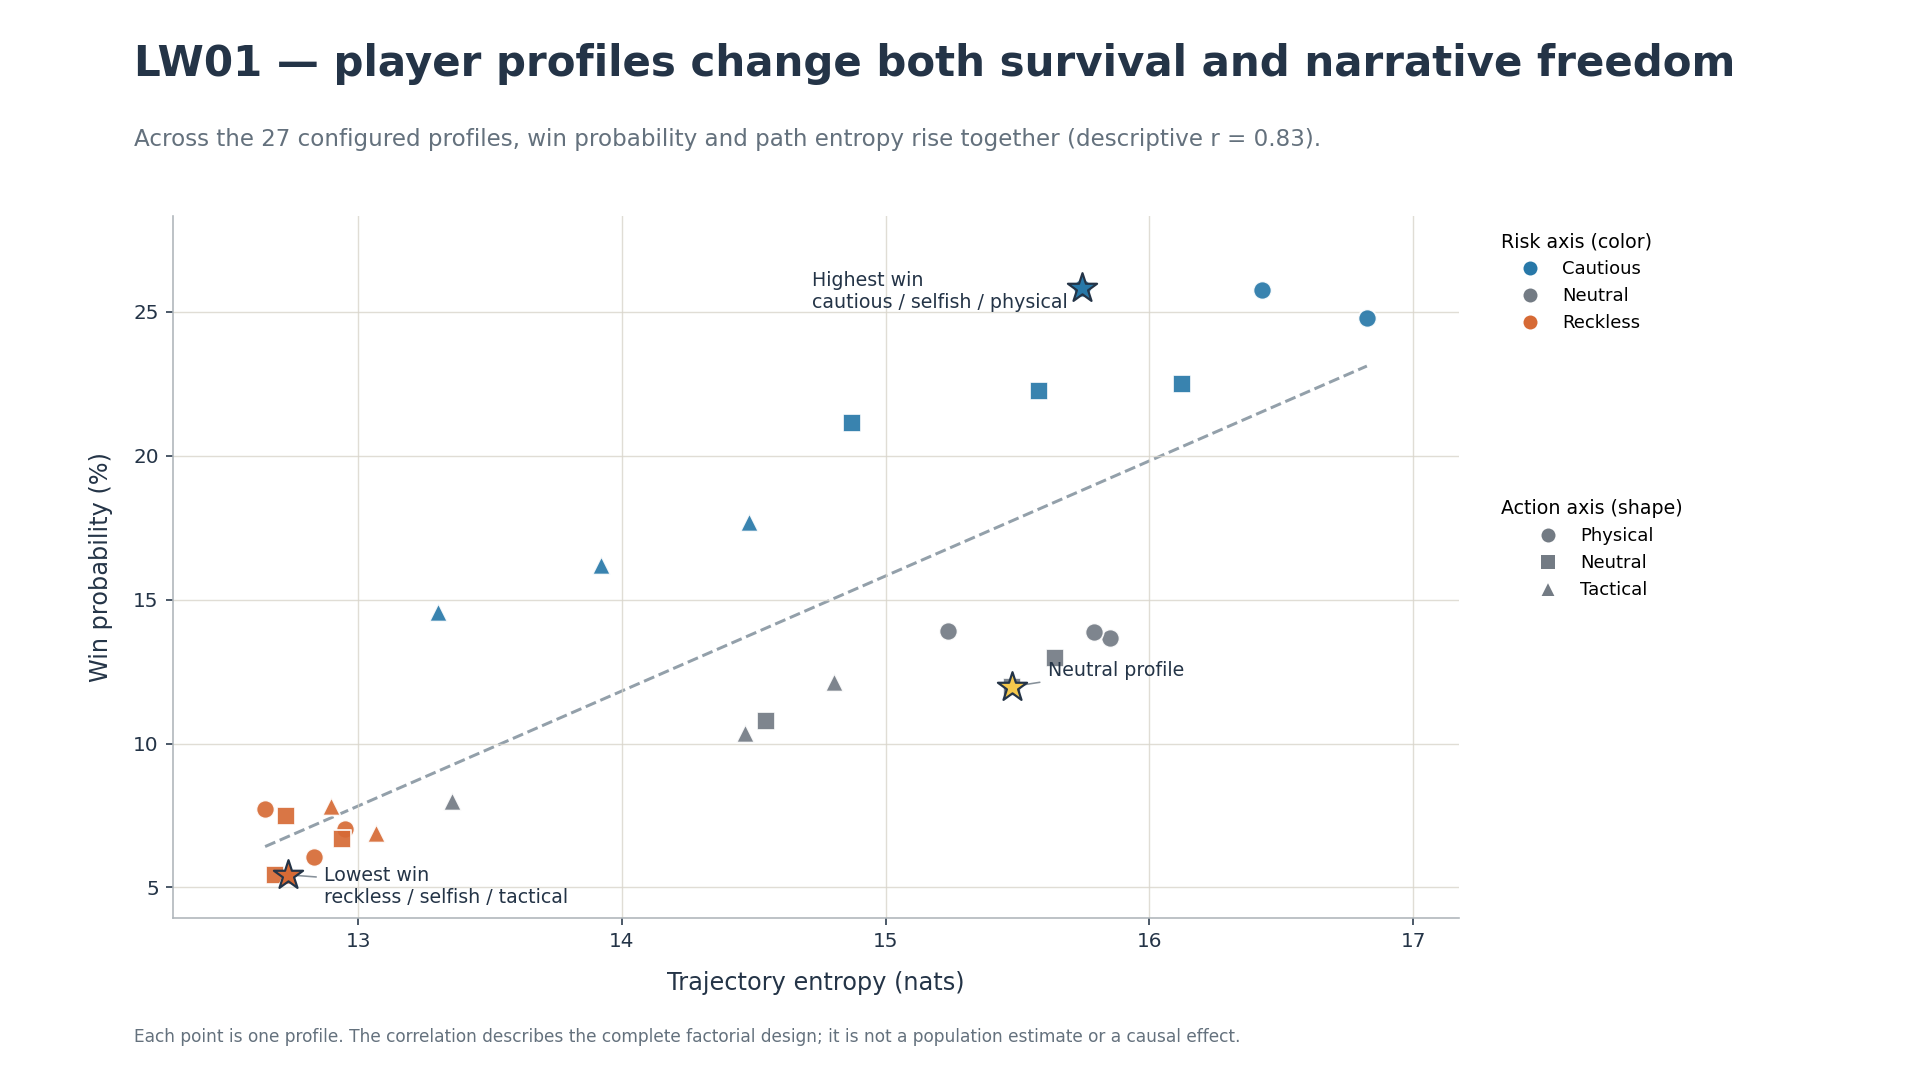
\includegraphics[width=\textwidth]{fig/01_profile_landscape.png}
		
		\vspace{-0.05cm}
		
		\begin{minipage}{0.94\textwidth}
			\scriptsize
			Across the \imp{27 configured profiles}, win probability ranges from
			\imp{5.4\% to 25.8\%}. Survival and trajectory entropy rise together
			($r=0.83$): profiles that survive longer also access a wider range of paths.
		\end{minipage}
		
	\end{frame}

	%-------------------------------------------%

	\begin{frame}{Risk is the dominant behavioral axis}
		
		\centering
		
		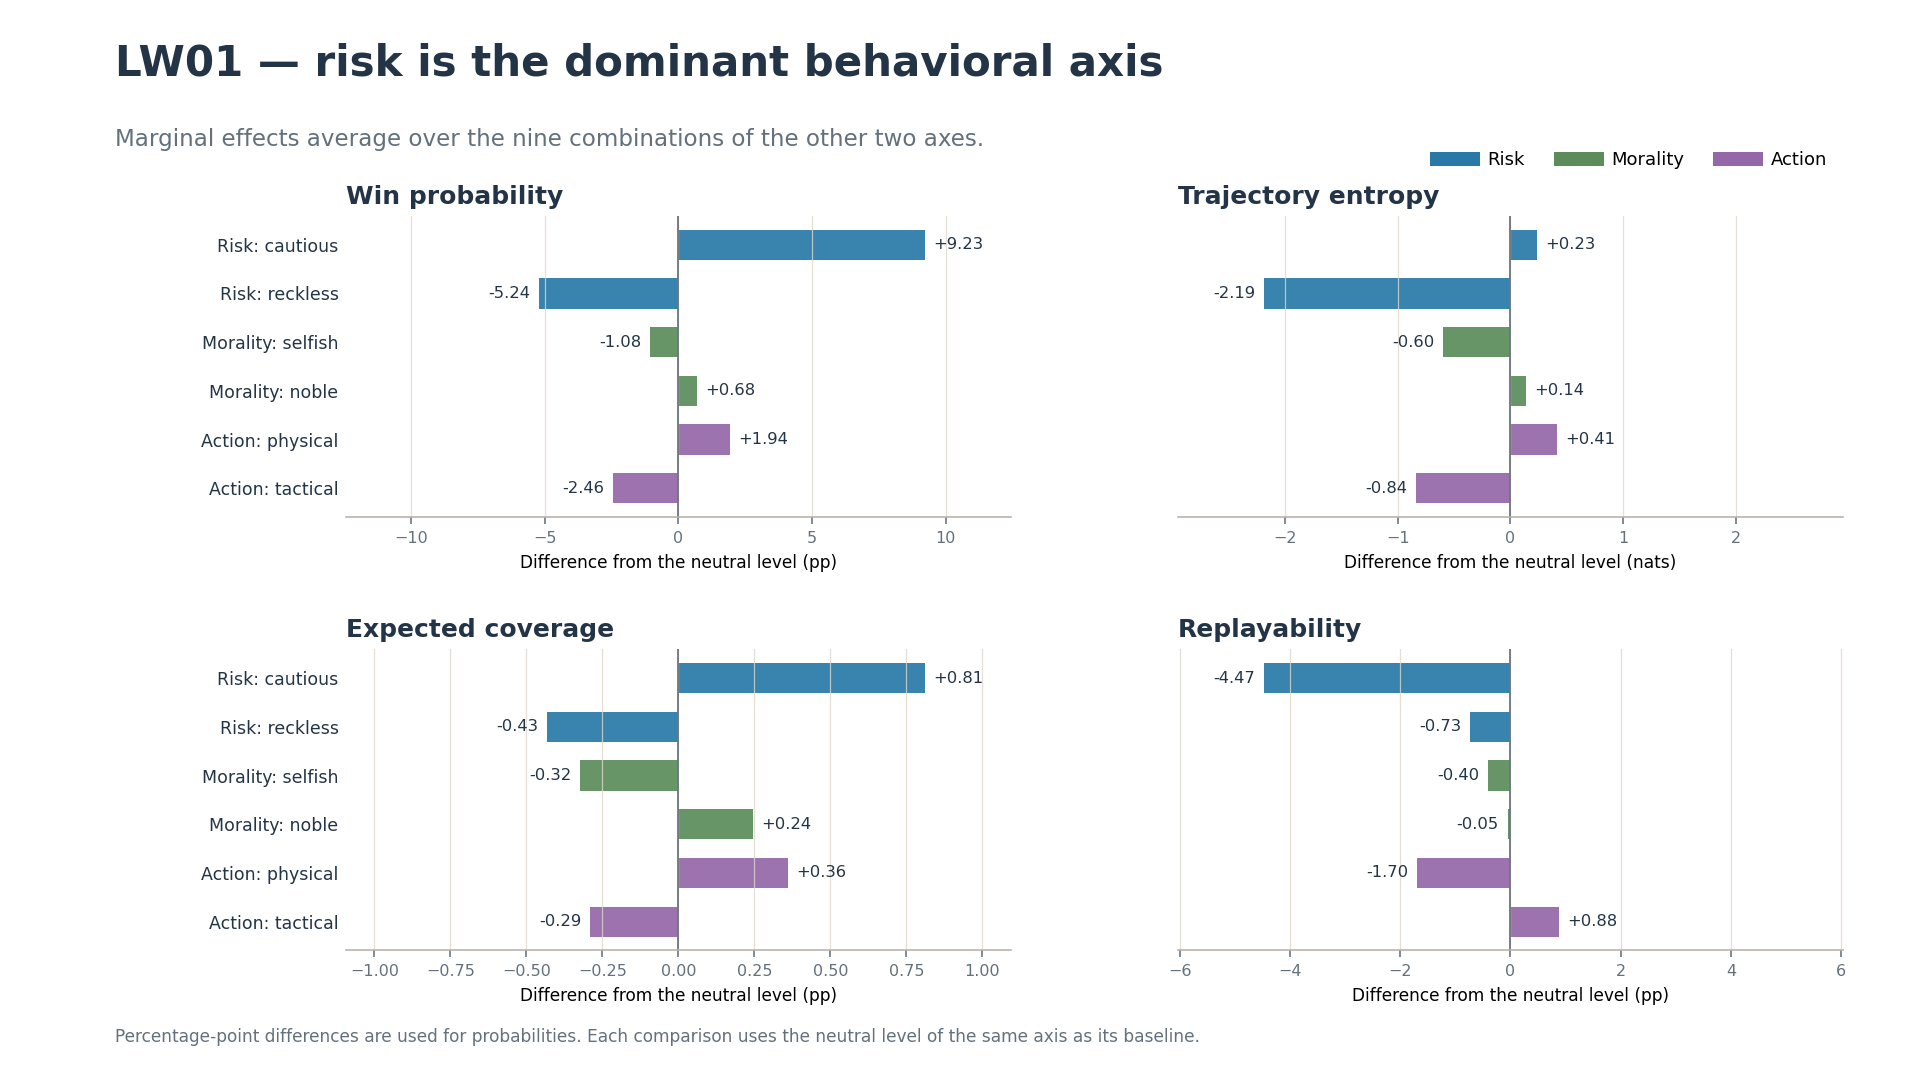
\includegraphics[width=\textwidth]{fig/02_axis_effects.png}
		
		\vspace{-0.05cm}
		
		\begin{minipage}{0.94\textwidth}
			\scriptsize
			Moving from neutral to cautious choices increases win probability by
			\imp{9.23 percentage points}; moving to reckless choices reduces it by
			\imp{5.24 points}. Morality and action have smaller, but non-zero, effects.
		\end{minipage}
		
	\end{frame}

	%-------------------------------------------%

	\begin{frame}{Different indices reveal different key paragraphs}
		
		\centering
		
		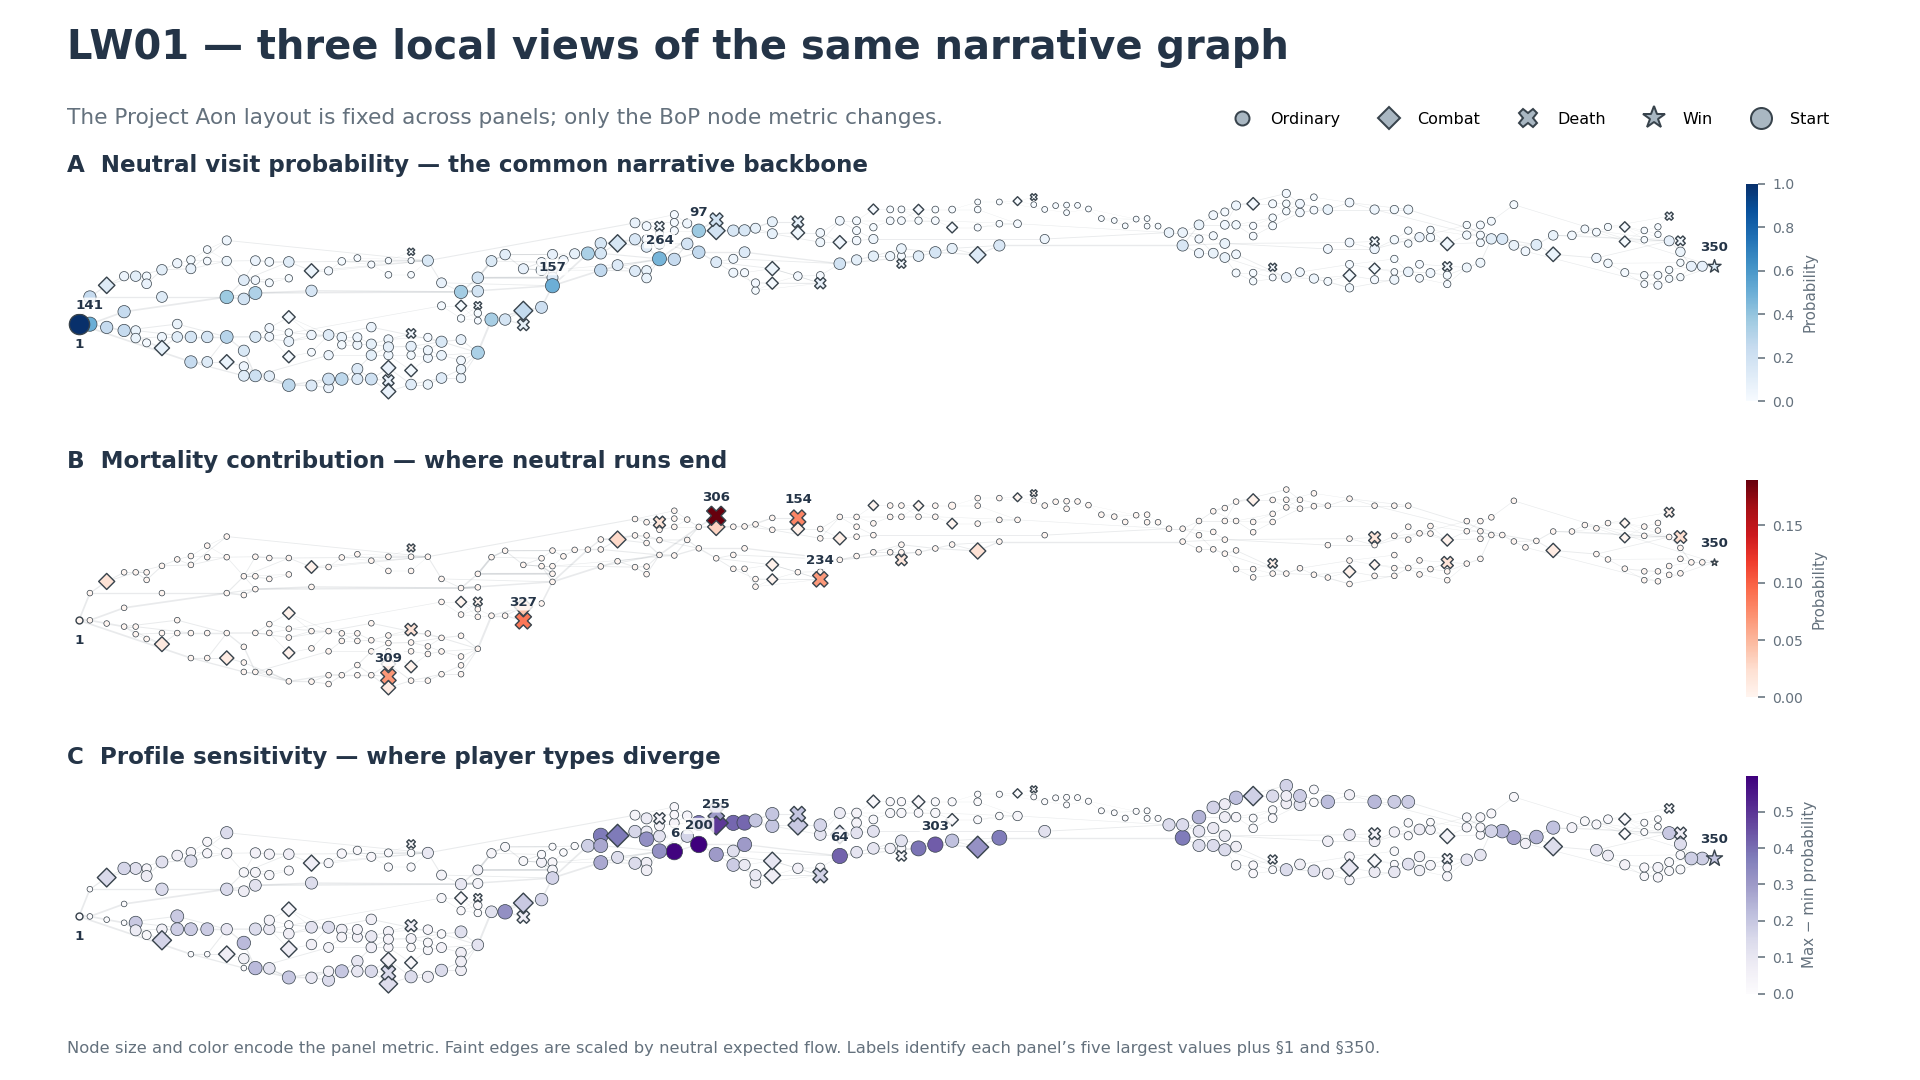
\includegraphics[width=\textwidth]{fig/03_local_index_maps.png}
		
		\vspace{-0.05cm}
		
		\begin{minipage}{0.94\textwidth}
			\scriptsize
			The common narrative backbone, the main mortality bottlenecks, and the
			regions where player profiles diverge \imp{do not coincide}. Local importance
			therefore depends on the structural question being asked.
		\end{minipage}
		
	\end{frame}

	%-------------------------------------------%

	\section{Trajectory annotation}

	%-------------------------------------------%

	\begin{frame}{Objective: from probabilistic paths to complete stories}
		
		\footnotesize
		
		This section asks whether the structural differences produced by player
		profiles become \imp{perceptible differences in complete stories}.
		
		\vspace{0.45cm}
		
		\centering
		
		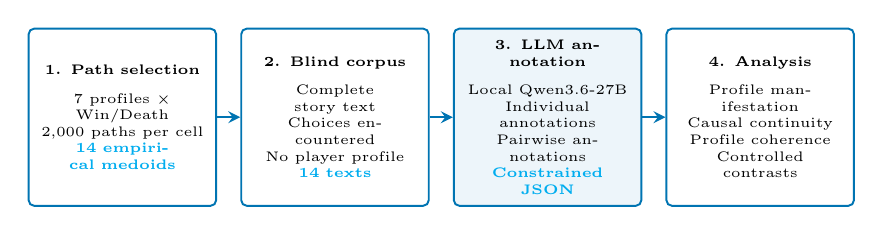
\begin{tikzpicture}[
			phasebox/.style={
				draw=themecolor,
				rounded corners=2pt,
				line width=0.7pt,
				fill=white,
				align=center,
				text width=2.10cm,
				minimum height=2.25cm,
				inner sep=4pt,
				font=\tiny
			},
			phasearrow/.style={
				->,
				>=stealth,
				draw=themecolor,
				line width=0.9pt
			}
		]
			
			\node[phasebox] (paths) at (-4.05,0) {
				\textbf{1. Path selection}\\[1.5mm]
				$7$ profiles $\times$ Win/Death\\
				2,000 paths per cell\\
				\imp{14 empirical medoids}
			};
			
			\node[phasebox] (corpus) at (-1.35,0) {
				\textbf{2. Blind corpus}\\[1.5mm]
				Complete story text\\
				Choices encountered\\
				No player profile\\
				\imp{14 texts}
			};
			
			\node[phasebox,fill=themecolor!7] (annotation) at (1.35,0) {
				\textbf{3. LLM annotation}\\[1.5mm]
				Local Qwen3.6-27B\\
				Individual annotations\\
				Pairwise annotations\\
				\imp{Constrained JSON}
			};
			
			\node[phasebox] (analysis) at (4.05,0) {
				\textbf{4. Analysis}\\[1.5mm]
				Profile manifestation\\
				Causal continuity\\
				Profile coherence\\
				Controlled contrasts
			};
			
			\draw[phasearrow] (paths.east) -- (corpus.west);
			\draw[phasearrow] (corpus.east) -- (annotation.west);
			\draw[phasearrow] (annotation.east) -- (analysis.west);
			
		\end{tikzpicture}
		
		\vspace{0.45cm}
		
		\raggedright
		The model infers whether the intended profile becomes perceptible from the
		story itself; the hidden metadata and BoP measures are reintroduced only for
		the final comparison.
		
	\end{frame}

	%-------------------------------------------%
	
	%-------------------------------------------%
	
	%-------------------------------------------%
	
	%-------------------------------------------%
	
	%-------------------------------------------%
	
	%-------------------------------------------%
	
\end{document}
